\documentclass[letterpaper, 10pt, conference]{ieeeconf}

\IEEEoverridecommandlockouts
\overrideIEEEmargins

\usepackage[T1]{fontenc}
\usepackage{amsmath,amsfonts}
\usepackage{graphicx}
\usepackage{booktabs}
\usepackage{multirow}
\usepackage[table]{xcolor}
\usepackage{cite}
\usepackage{url}
\usepackage{array}

\title{\LARGE \bf Geometry-Guided Feed-Forward Regression for\\LiDAR-Inertial-Camera Photo-Realistic 2DGS Mapping}

\author{Author Names Omitted for Review}

\begin{document}

\maketitle
\thispagestyle{empty}
\pagestyle{empty}

%%%%%%%%%%%%%%%%%%%%%%%%%%%%%%%%%%%%%%%%%%%%%%%%%%%%%%%%%%%%%%%%%%%%%%%%%%%%%%%%
% ABSTRACT
%%%%%%%%%%%%%%%%%%%%%%%%%%%%%%%%%%%%%%%%%%%%%%%%%%%%%%%%%%%%%%%%%%%%%%%%%%%%%%%%

\begin{abstract}

Incremental 3D scene reconstruction requires the system to continuously expand the map while receiving observations frame by frame. The limited online optimization budget makes the initial attribute quality of newly inserted Gaussians directly affect the cumulative mapping result. Existing incremental mapping systems based on 3D Gaussian Splatting (3DGS) have two interrelated limitations: 3D ellipsoidal primitives lack explicit surface normal semantics, and rule-based initialization strategies fail to fully exploit external geometric priors. We propose a context-aware feed-forward Gaussian regression system for incremental 2D Gaussian Splatting (2DGS) scene reconstruction. The system adopts 2DGS surfels as the map representation and combines depth completion with monocular normal priors to construct candidate points with geometric orientations. A feed-forward regression network aggregates image-rendering context from the current and historical frames via cross-attention, anchors surfel rotation on normal priors through Gram-Schmidt orthogonalization, and predicts complete surfel attributes in a single forward pass. The network is trained through self-distillation without any external annotated dataset. Experiments on the R3LIVE and MCD datasets show that our method outperforms all baselines on every test sequence, achieving an average improvement of 1.28\,dB PSNR over the closest multi-sensor incremental Gaussian mapping baseline. Ablation studies further confirm that the feed-forward regressor consistently improves the early convergence quality of new Gaussians under limited optimization budgets.

\end{abstract}

%%%%%%%%%%%%%%%%%%%%%%%%%%%%%%%%%%%%%%%%%%%%%%%%%%%%%%%%%%%%%%%%%%%%%%%%%%%%%%%%
% I. INTRODUCTION
%%%%%%%%%%%%%%%%%%%%%%%%%%%%%%%%%%%%%%%%%%%%%%%%%%%%%%%%%%%%%%%%%%%%%%%%%%%%%%%%

\section{INTRODUCTION}

Incremental 3D scene reconstruction is essential for time-critical field operations such as disaster response, autonomous driving, and industrial inspection. Recent incremental Gaussian mapping systems that fuse LiDAR, inertial, and visual measurements have demonstrated online photo-realistic reconstruction in large-scale outdoor environments: an external front-end provides stable poses and multi-modal observations, while a Gaussian back-end expands the map frame by frame with Gaussian primitives. However, the per-frame optimization budget of an online system is inherently limited. Newly inserted Gaussians undergo only a few optimization steps before they must serve subsequent rendering, so their initial attribute quality directly affects the cumulative mapping result.

Existing systems still have interrelated limitations in both map representation and initialization. On the representation side, standard 3DGS~\cite{kerbl20233d} uses 3D ellipsoids as primitives that lack explicit surface normal semantics, preventing direct coupling between geometric priors and the map. 2DGS~\cite{huang20242d} achieves notable geometric improvements by collapsing Gaussians into oriented 2D disks, yet it has not been adopted in incremental mapping. On the initialization side, existing systems predominantly assign attributes to new Gaussians through rule-based strategies, requiring many optimization steps to converge and conflicting with the limited per-frame budget. Although some systems introduce depth completion to address sparse LiDAR coverage, learned priors serve only for point placement and have not been extended to full attribute prediction. Without geometric interpretability in the representation, rule-based initialization cannot effectively leverage external priors; without learned attribute prediction, the advantages of surface-based representations cannot be realized at insertion time.

We propose a context-aware feed-forward Gaussian regression system for incremental 2DGS scene reconstruction. The system adopts 2DGS surfels as the map representation. Given poses from an external LiDAR-inertial-visual (LIVO) front-end, it fuses depth completion and monocular normal priors to construct candidate points with geometric orientations. A feed-forward regression network aggregates image-rendering context from the current frame and historical frames within a sliding window, predicting complete surfel attributes for new Gaussians in a single forward pass before they enter online optimization. The network is trained through a self-distillation procedure that requires no external annotated dataset.

The main contributions are as follows:

\begin{itemize}
    \item A geometry-aware incremental Gaussian map back-end based on 2DGS surfels. Unlike existing incremental systems that default to 3DGS volumetric Gaussians, the surface-based 2DGS representation endows the map with explicit normal semantics, enabling direct coupling of depth completion and normal priors and providing a geometrically interpretable foundation for feed-forward initialization.

    \item A context-aware feed-forward Gaussian insertion method. Rather than assigning attributes through per-point rules, our network aggregates multi-view context via per-point cross-attention and anchors predictions on normal priors, predicting complete surfel attributes in a single forward pass so that new Gaussians are closer to convergence at insertion and early quality loss under limited optimization budgets is significantly reduced.

    \item A self-distillation training procedure for the feed-forward network that collects supervision signals solely from the system's own incremental mapping process on training scenes, requiring no external annotated dataset.
\end{itemize}

%%%%%%%%%%%%%%%%%%%%%%%%%%%%%%%%%%%%%%%%%%%%%%%%%%%%%%%%%%%%%%%%%%%%%%%%%%%%%%%%
% II. RELATED WORK
%%%%%%%%%%%%%%%%%%%%%%%%%%%%%%%%%%%%%%%%%%%%%%%%%%%%%%%%%%%%%%%%%%%%%%%%%%%%%%%%

\begin{figure*}[!t]
    \centering
    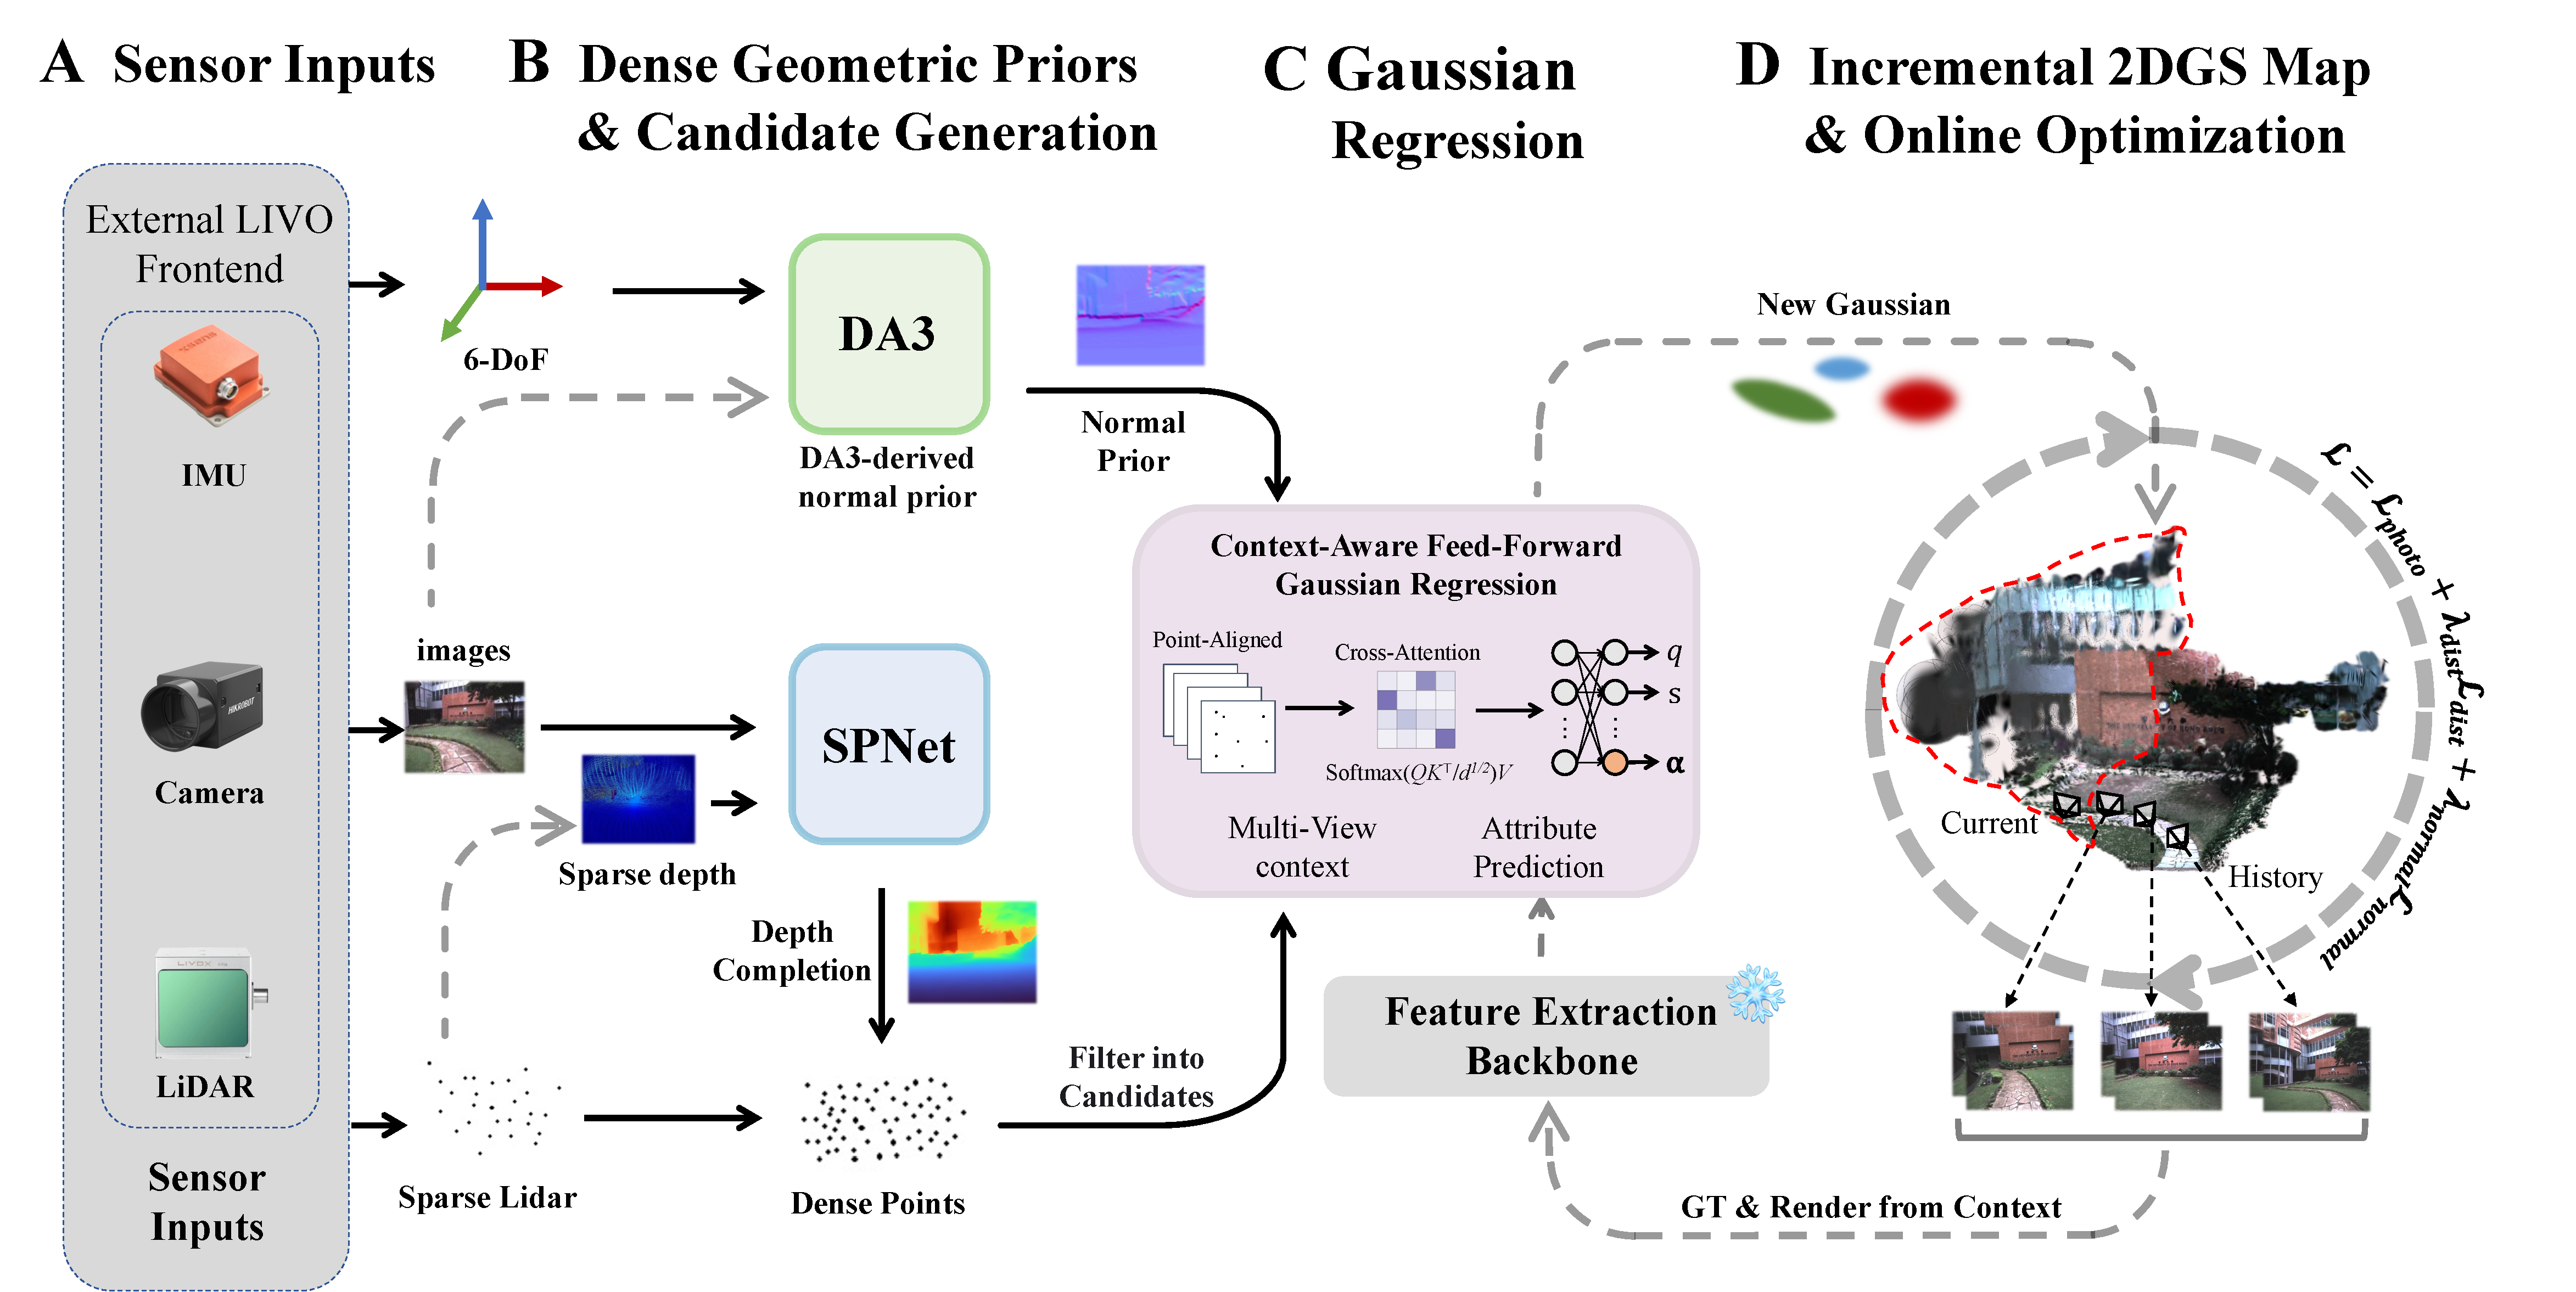
\includegraphics[width=\textwidth,height=0.36\textheight,keepaspectratio]{../system-pipeline.pdf}
    \caption{System pipeline. (A) An external LiDAR-inertial-visual front-end provides synchronized RGB images, LiDAR observations, IMU measurements, and camera poses. (B) The system generates dense geometric priors via SPNet depth completion and DA3 normal estimation, which together with LiDAR points form initial points in under-reconstructed regions. (C) For each candidate point, the feed-forward Gaussian regressor aggregates point-aligned multi-view context and directly predicts 2DGS surfel attributes. (D) The predicted new surfels are inserted into the incremental map and further refined by online optimization; the current map renderings in turn serve as context input for subsequent insertions.}
    \label{fig:system_pipeline}
\end{figure*}

\section{RELATED WORK}

NeRF~\cite{mildenhall2021nerf} and its follow-up works have demonstrated the advantages of radiance field representations for novel view synthesis and continuous appearance modeling, yet the costly sampling and integration inherent in volume rendering make it difficult to meet the demands of real-time incremental reconstruction. 3D Gaussian Splatting (3DGS)~\cite{kerbl20233d} replaces volume integration with explicit Gaussian primitives and differentiable rasterization, achieving clear advantages in rendering speed and optimization efficiency that quickly make it an important foundation for online photo-realistic mapping.

Research around 3DGS advances along two directions. One line of work targets geometric quality: 2DGS~\cite{huang20242d}, GaussianSurfels~\cite{dai2024high}, and PGSR~\cite{chen2024pgsr} improve geometric consistency through surface-oriented Gaussians, depth rasterization, and normal constraints. These methods show that explicit surface orientation is better suited than 3D ellipsoids for carrying depth and normal priors, a property that is particularly relevant for incremental systems. Another line of work targets feed-forward Gaussian priors: pixelSplat~\cite{charatan2024pixelsplat} and MVSplat~\cite{chen2024mvsplat} predict generalizable Gaussian representations from a small number of input images via probabilistic sampling or cost-volume mechanisms. Although these methods primarily address offline or one-shot multi-view reconstruction, the geometric and appearance priors embodied in their outputs open new possibilities for initialization and completion in online systems.

In online mapping, MonoGS~\cite{matsuki2024gaussian}, GS-SLAM~\cite{yan2024gs}, SplaTAM~\cite{keetha2024splatam}, and Photo-SLAM~\cite{huang2024photo} have demonstrated that 3DGS can serve as the unified map representation for monocular online systems, coupling tracking, mapping, and rendering on a single Gaussian map, but these works target only indoor scenes. For large-scale outdoor environments, LiDAR-inertial-camera fusion provides more stable poses and geometric observations. Gaussian-LIC~\cite{lang2024gaussian} initializes a 3DGS map from LiDAR points and visual triangulation. GS-LIVM~\cite{xie2024gs} and GS-LIVO~\cite{hong2025gs} further address sparse LiDAR coverage, local window optimization, and resource constraints. Gaussian-LIC2~\cite{lang2025gaussianlic2} introduces depth completion priors to improve Gaussian initialization. These works are closest to our problem setting, yet they still primarily adopt a 3DGS back-end, and learned priors are mostly limited to point placement or depth completion rather than predicting complete attributes such as scale, orientation, color, and opacity. We adopt 2DGS surfels as the map representation under LIVO-provided poses and predict complete new surfel attributes through a feed-forward network, thereby improving the initial quality at the incremental insertion stage.

%%%%%%%%%%%%%%%%%%%%%%%%%%%%%%%%%%%%%%%%%%%%%%%%%%%%%%%%%%%%%%%%%%%%%%%%%%%%%%%%
% III. METHOD
%%%%%%%%%%%%%%%%%%%%%%%%%%%%%%%%%%%%%%%%%%%%%%%%%%%%%%%%%%%%%%%%%%%%%%%%%%%%%%%%

\section{METHOD}

\subsection{System Overview}

The proposed system is an incremental 2DGS scene reconstruction back-end that relies on external pose estimation. It receives a synchronized data stream from an external LiDAR-inertial-camera front-end (e.g., R3Live~\cite{lin2022r}), where each frame contains an RGB image, a sparse LiDAR point cloud, and a 6-DoF camera pose, and uses 2DGS surfels as the fundamental map representation. The overall pipeline is illustrated in Fig.~\ref{fig:system_pipeline}.

When a new keyframe arrives, the system first refines its camera pose by rendering the existing Gaussians onto the current frame and minimizing the photometric error. It then inserts new Gaussians and optimizes existing ones. Sparse LiDAR points are projected onto the image plane to form a sparse depth map, which is densified by SPNet~\cite{li2023spnet} depth completion to produce supplementary 3D points in LiDAR-blind regions. Concurrently, the DA3~\cite{lin2025da3} monocular depth model predicts dense relative depth and is aligned to absolute scale via least-squares affine registration with the sparse LiDAR depth, from which per-pixel normals are derived. After the initial points are generated, the system renders the current Gaussian map and identifies under-reconstructed regions based on rendering transmittance and color error. Color-gradient filtering and voxel downsampling further select the subset of candidate points that genuinely require new Gaussians. The system then uses these candidates as a mask to filter the feature maps and normal maps, extracting point-aligned features that form the two inputs to the feed-forward regression network: context features $\mathbf{ctx}$ and geometric priors $\mathbf{g}$. The network aggregates multi-view context via cross-attention and regresses complete surfel attributes for each candidate in a single forward pass. The resulting high-quality new Gaussians are inserted into the map. Online optimization then follows on sampled keyframes, jointly driven by photometric loss $\mathcal{L}_{\text{photo}}$ and geometric constraints ($\mathcal{L}_{\text{dist}}$ and $\mathcal{L}_{\text{normal}}$). Non-keyframes receive only pose updates without triggering Gaussian insertion.

The feed-forward regression network is trained via self-distillation without any external annotated data. The key idea is to construct supervision signals from the system's own online-optimized Gaussian results on training scenes, enabling the network to learn a better surfel initialization strategy.

\subsection{Dense Geometric Priors}

We employ the lightweight SPNet~\cite{li2023spnet} depth completion network to fuse the RGB image with sparse LiDAR depth into a dense depth map and sample supplementary 3D points in regions lacking LiDAR coverage. The SPNet-complemented points are merged with the original LiDAR projection points to form the initial point set.

Compared with normals obtained by directly differentiating the SPNet-completed depth, the DA3 model~\cite{lin2025da3} possesses stronger scene-structure priors and produces smoother, more stable surface orientation estimates. We therefore run DA3 on the current RGB frame to obtain a relative depth map, register it to the sparse LiDAR depth via least-squares affine alignment to recover metric scale, and compute per-pixel normals by central differencing. Sampling the normal map at the pixel coordinates of the initial points yields a camera-space normal $\mathbf{n}_{\text{cam}} \in \mathbb{R}^3$ for each point.

\subsection{Feed-Forward Gaussian Regression Network}

\begin{figure*}[!t]
    \centering
    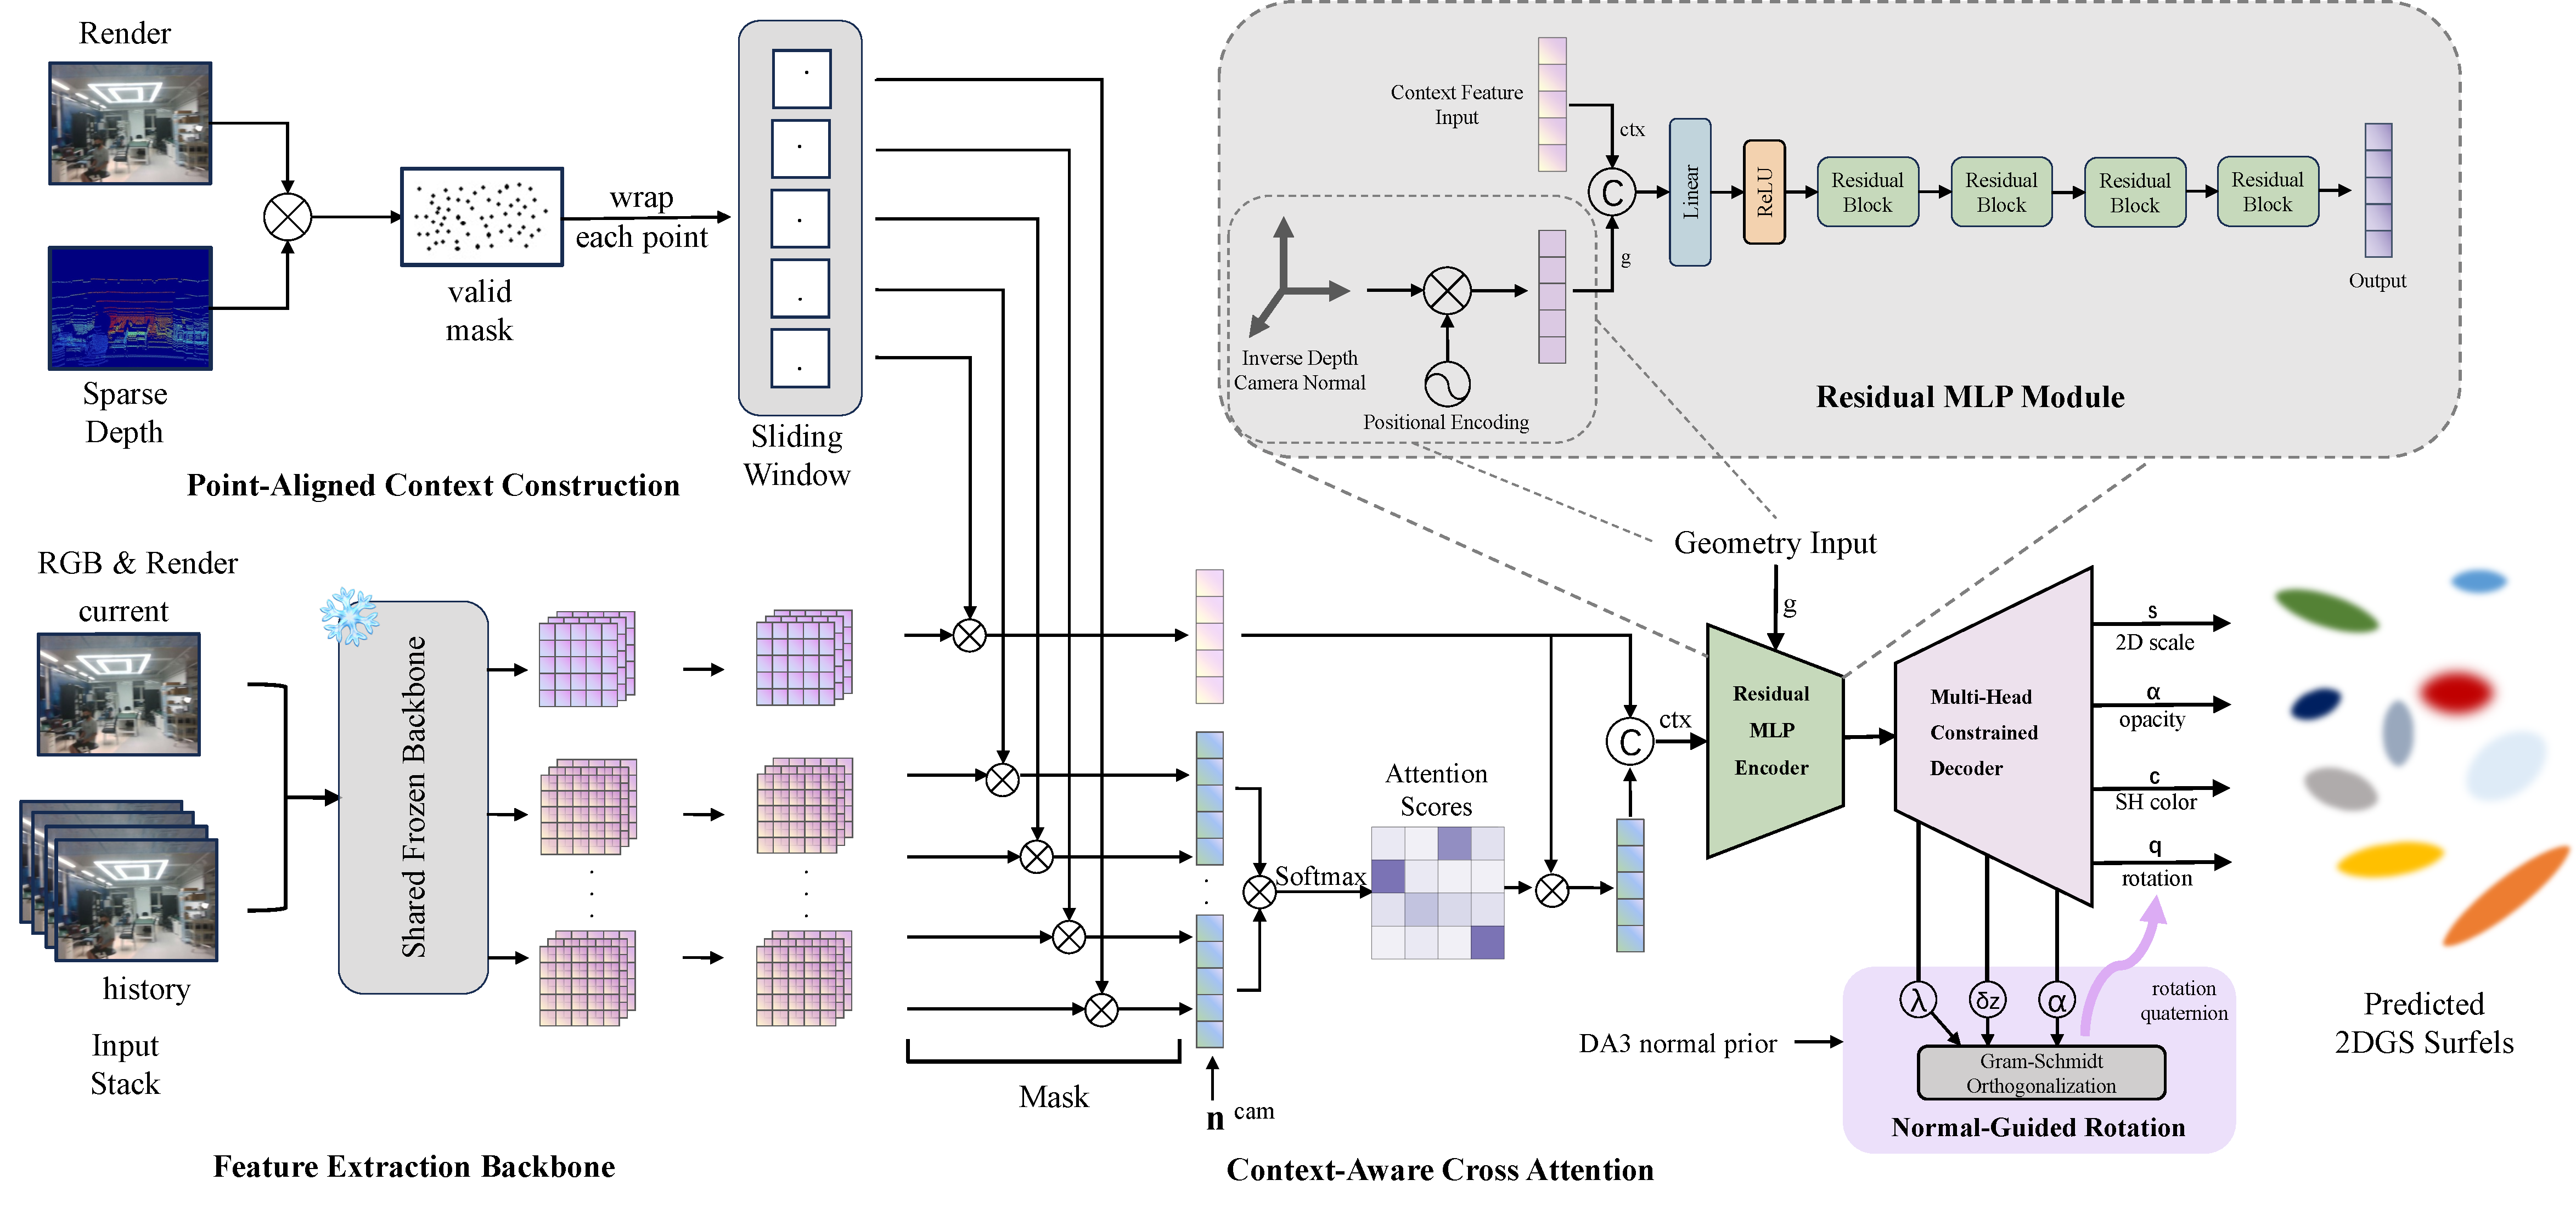
\includegraphics[width=\textwidth,height=0.42\textheight,keepaspectratio]{../net-pipeline.pdf}
    \caption{Architecture of the context-aware feed-forward Gaussian regressor. The network first constructs point-aligned context for valid candidate points within a sliding window and extracts image-rendering features from the current and historical frames through a frozen shared backbone. A cross-attention module then aggregates multi-view appearance information, which is fed together with inverse depth, DA3 normals, and positional encodings into a residual MLP encoder. Finally, a multi-head constrained decoder predicts the 2DGS surfel attributes $(s, \alpha, c, q)$, where the normal-guided rotation branch constructs a geometrically consistent orientation via Gram-Schmidt orthogonalization.}
    \label{fig:net-pipeline}
\end{figure*}

As illustrated in Fig.~\ref{fig:net-pipeline}, the feed-forward Gaussian regressor organizes its input and prediction around candidate points. The system first locates under-reconstructed regions from the current map's $\alpha$-blending result and filters the depth-completion output accordingly to obtain the candidate points for the current keyframe. For each candidate, multi-view context features are aggregated and combined with geometric priors; a shared encoder and multi-head decoder then output the complete surfel attributes. Unlike methods such as MVSplat~\cite{chen2024mvsplat} that predict Gaussian parameters densely on an image grid, the candidate points in our setting are already determined by upstream geometric modules. The goal is therefore not to learn a dense pixel-aligned mapping from multi-view images to surfels, but rather, for each of the $N_t$ candidate points selected in the current keyframe, to sample and aggregate point-aligned context from multi-view feature maps and learn a mapping from the context features $\mathbf{ctx}$ and geometric priors $\mathbf{g}$ to surfel parameters. Denoting $\mathbf{ctx}_i$ and $\mathbf{g}_i$ as the context and geometric-prior inputs for candidate $i$, the feed-forward network can be written as:
%
\begin{equation}
f_{\boldsymbol{\theta}} : \{(\mathbf{ctx}_i, \mathbf{g}_i)\}_{i=1}^{N_t}
\mapsto
\{(\mathbf{s}_i, \mathbf{q}_i, \alpha_i, \mathbf{c}_i^{\mathrm{dc}}, \mathbf{c}_i^{\mathrm{rest}})\}_{i=1}^{N_t},
\end{equation}
%
where the outputs correspond to the 2D scale, rotation, opacity, and SH color coefficients of each surfel.

\vspace{0.35em}
\noindent 1) Context feature input $\mathbf{ctx}$: A shared backbone (following the pixelSplat~\cite{charatan2024pixelsplat} design, frozen during training) extracts feature maps from the current-frame raw image, the current-frame rendered image, and the raw and rendered images of $W$ historical keyframes within a sliding window. Historical keyframes are introduced because a single viewpoint provides insufficient constraints for surfel attribute regression; rendered images allow the regressor to perceive the current reconstruction state explicitly, and their difference from raw images implicitly reflects the degree of under-reconstruction. For each candidate point, the system projects it onto the current frame and each historical keyframe, performs bilinear interpolation on the corresponding feature maps, and computes the normalized viewing direction. The raw-image features, rendered-image features, and encoded viewing-direction vectors are concatenated to form the per-point current-frame feature $\mathbf{f}_i^{\text{curr}} \in \mathbb{R}^{D}$. The same procedure is applied to the $W$ visible historical frames, yielding $\mathbf{f}_i^{\text{hist}} \in \mathbb{R}^{W \times D}$, with a visibility mask $\mathbf{m}_i^{\text{hist}} \in \{0,1\}^{W}$ marking occluded views. A cross-attention module then compresses the variable-length historical observations into a fixed-dimensional temporal context, where invisible views are excluded by a $-\infty$ mask before the softmax:
%
\begin{equation}
\mathbf{ctx}_i^{\text{attn}} = \text{softmax}\!\left(\frac{\mathbf{q}_i \mathbf{K}_i^\top}{\sqrt{d_k}} + \mathbf{M}_i\right) \mathbf{V}_i.
\end{equation}
%
The current-frame feature $\mathbf{f}_i^{\text{curr}}$ and the attention output $\mathbf{ctx}_i^{\text{attn}}$ are concatenated to form the encoder input $\hat{\mathbf{ctx}}_i$.

\vspace{0.35em}
\noindent 2) Geometric prior input $\mathbf{g}$: The geometric prior is the concatenation of inverse depth, the DA3 camera-space normal, a validity mask, and the KNN pixel spacing:
%
\begin{equation}
\mathbf{g}_i = [\bar{z}_i^{-1} \| \mathbf{n}_i^{\text{cam}} \| m_i \| d_i^{\text{nn}}].
\end{equation}
%
Here $\bar{z}_i^{-1}$ provides the depth information needed for scale recovery, $\mathbf{n}_i^{\text{cam}}$ serves as the normal anchor for surfel orientation, $m_i$ flags whether the geometric prior is valid, and $d_i^{\text{nn}}$ captures the local sampling density. Each continuous component undergoes NeRF-style positional encoding and is concatenated with $\hat{\mathbf{ctx}}_i$ before being fed into the encoder, which consists of one linear projection followed by four pre-activation residual blocks and outputs a 512-dimensional latent vector $\mathbf{h}_i$.

\vspace{0.35em}
\noindent 3) Decoder: On top of the shared latent $\mathbf{h}_i$, separate prediction heads of the form Linear $\to$ ReLU $\to$ Linear regress different attributes. Each head output is not used directly as the final Gaussian parameter but is decoded through upstream geometric priors, anchoring predictions on existing geometric information for greater stability.

\vspace{0.25em}
\noindent a) Normal-guided rotation decoding. Rather than regressing a quaternion directly, the system takes the DA3 camera-space normal $\mathbf{n}_i^{\text{cam}}$ as an anchor and lets the network predict a correction. The network outputs a normal correction vector $\delta \mathbf{z}_i \in \mathbb{R}^3$, a blending strength $\lambda_i = \text{softplus}(\cdot) \in \mathbb{R}_{>0}$, and an auxiliary vector $\mathbf{a}_i \in \mathbb{R}^3$, from which the corrected normal direction is obtained:
%
\begin{equation}
\mathbf{z}_i = \text{normalize}(\mathbf{n}_i^{\text{cam}} + \lambda_i \cdot \delta \mathbf{z}_i).
\end{equation}
%
A full orthonormal basis is then constructed via Gram-Schmidt orthogonalization:
%
\begin{equation}
\mathbf{y}_i = \text{normalize}(\mathbf{z}_i \times \mathbf{a}_i), \qquad \mathbf{x}_i = \mathbf{y}_i \times \mathbf{z}_i.
\end{equation}
%
The camera-frame rotation matrix $[\mathbf{x}_i \mid \mathbf{y}_i \mid \mathbf{z}_i]$ is transformed to the world frame through the current pose $R_{\text{wc}}$ and stored as a unit quaternion.

\vspace{0.25em}
\noindent b) Density-adaptive scale decoding. The scale head predicts the relative surfel size in the pixel plane, modulated by the local point-density prior:
%
\begin{equation}
\mathbf{s}_i^{\text{pixel}} = \frac{d_i^{\text{nn}}}{2} \cdot \exp(\text{head}(\mathbf{h}_i)) \in \mathbb{R}^2_{>0},
\end{equation}
%
where $d_i^{\text{nn}}$ is the KNN pixel spacing of the candidate point. The world-space scale is recovered by
%
\begin{equation}
\mathbf{s}_i^{\text{world}} = \mathbf{s}_i^{\text{pixel}} / (\bar{z}_i^{-1} \cdot f).
\end{equation}
%
This parameterization avoids requiring the network to learn depth-dependent absolute scales and instead only learns relative scale variations related to local density.

\vspace{0.25em}
\noindent c) Color decoding. The DC color head outputs a residual $\Delta \mathbf{c}_i^{\text{dc}}$ that is added to a base SH prior converted from the single-frame RGB observation:
%
\begin{equation}
\mathbf{c}_i^{\text{dc}} = \text{RGB2SH}(\mathbf{I}_i) + \Delta \mathbf{c}_i^{\text{dc}}.
\end{equation}
%
Higher-order SH coefficients are predicted by a separate head. The residual design lets the network start from a reasonable color prior and learn only local corrections.

\vspace{0.25em}
\noindent d) Opacity decoding. The opacity head applies a sigmoid activation to produce $\alpha_i \in (0,1)$, which is then converted to logit space for storage.

\subsection{Self-Distillation Training}

The feed-forward network is trained without any external multi-view annotated dataset through the following self-distillation pipeline.

\vspace{0.35em}
\noindent 1) Online data collection. The system first runs a complete incremental mapping pass on training scenes in a naive mode that does not use the feed-forward network but instead applies rule-based initialization. During this pass, when the cumulative training count of a frame's newly added Gaussians reaches a preset threshold, the system snapshots their current attributes as supervision signals and simultaneously projects them into the current sliding window to construct the corresponding context features $\mathbf{ctx}_i$ and geometric priors $\mathbf{g}_i$ following the definitions above. Each training sample is thus organized as the input-output pair $(\mathbf{ctx}_i, \mathbf{g}_i) \mapsto (\mathbf{s}_i, \mathbf{q}_i, \alpha_i, \mathbf{c}_i^{\mathrm{dc}}, \mathbf{c}_i^{\mathrm{rest}})$.

\vspace{0.35em}
\noindent 2) Scale-rotation ambiguity resolution. A 2DGS surfel has an inherent scale-rotation ambiguity: swapping the two tangent-direction scales and rotating by $90^\circ$ yields an equivalent representation. If unresolved, the same geometry maps to two different parameter combinations in the training labels, destabilizing learning. During data preparation, this ambiguity is explicitly resolved: for each ground-truth Gaussian, $s_1 \geq s_2$ is enforced; when a swap is needed, the quaternion is simultaneously rotated by $90^\circ$: $\mathbf{q}' = \text{normalize}((w{-}z,\; x{+}y,\; y{-}x,\; w{+}z) / \sqrt{2})$.

\vspace{0.35em}
\noindent 3) Training objective. The network is trained with a multi-task loss covering all predicted attributes. Scale loss is measured by L1 distance in log world-scale space. Rotation loss uses the quaternion cosine distance $\mathcal{L}_{\text{rot}} = 1 - |\langle \mathbf{q}_{\text{pred}}, \mathbf{q}_{\text{gt}} \rangle|$. Color losses supervise DC and higher-order SH coefficients separately with MSE. Opacity loss is an L1 distance.

%%%%%%%%%%%%%%%%%%%%%%%%%%%%%%%%%%%%%%%%%%%%%%%%%%%%%%%%%%%%%%%%%%%%%%%%%%%%%%%%
% IV. EXPERIMENTAL RESULTS
%%%%%%%%%%%%%%%%%%%%%%%%%%%%%%%%%%%%%%%%%%%%%%%%%%%%%%%%%%%%%%%%%%%%%%%%%%%%%%%%

\section{EXPERIMENTAL RESULTS}

\begin{table*}[!t]
\centering
\caption{Novel-view RGB rendering results on R3LIVE (Avia), MCD (OS1-64), and self-collected campus datasets. Format: PSNR$\uparrow$ $|$ SSIM$\uparrow$ $|$ LPIPS$\downarrow$. Best results in bold.}
\label{tab:r3live_rendering}
\renewcommand{\arraystretch}{1.15}
\setlength{\tabcolsep}{8pt}
\resizebox{\textwidth}{!}{%
\begin{tabular}{lcccc}
\toprule
\textbf{Sequence} & \multicolumn{4}{c}{\textbf{Rendering Quality (PSNR$\uparrow$ $|$ SSIM$\uparrow$ $|$ LPIPS$\downarrow$)}} \\
\cmidrule(lr){2-5}
& \textbf{MonoGS~\cite{matsuki2024gaussian}} & \textbf{MM3DGS-SLAM~\cite{sun2024mm3dgs}} & \textbf{Gaussian-LIC2~\cite{lang2025gaussianlic2}} & \textbf{Ours} \\
\midrule
\rowcolor{black!8}
\multicolumn{5}{l}{\textbf{R3LIVE (Avia)}} \\
degenerate\_seq\_00 & 14.59 | 0.460 | 0.624 & 19.35 | 0.698 | 0.212 & 21.99 | 0.782 | 0.162 & \textbf{23.41} | \textbf{0.821} | \textbf{0.137} \\
degenerate\_seq\_01 & 14.66 | 0.438 | 0.692 & 18.57 | 0.621 | 0.277 & 22.94 | 0.790 | 0.159 & \textbf{23.54} | \textbf{0.810} | \textbf{0.157} \\
hku\_campus\_00 & 15.41 | 0.464 | 0.675 & 18.70 | 0.621 | 0.319 & 24.34 | 0.787 | 0.156 & \textbf{25.52} | \textbf{0.820} | \textbf{0.152} \\
hku\_campus\_01 & 8.39 | 0.065 | 0.873 & 16.97 | 0.593 | 0.271 & 20.52 | 0.674 | 0.236 & \textbf{23.15} | \textbf{0.754} | \textbf{0.174} \\
hku\_park\_00 & 13.24 | 0.319 | 0.733 & 14.98 | 0.363 | 0.396 & 17.17 | 0.469 | 0.340 & \textbf{17.80} | \textbf{0.491} | \textbf{0.331} \\
hku\_park\_01 & 12.22 | 0.289 | 0.790 & 15.79 | 0.392 | 0.409 & 19.46 | 0.529 | 0.325 & \textbf{20.65} | \textbf{0.580} | \textbf{0.248} \\
\rowcolor{black!8}
\multicolumn{5}{l}{\textbf{MCD (OS1-64)}} \\
tuhh\_day\_02 & 8.72 | 0.158 | 0.893 & 11.15 | 0.478 | 0.350 & 20.35 | 0.626 | 0.262 & \textbf{20.99} | \textbf{0.652} | \textbf{0.249} \\
tuhh\_day\_03 & 8.09 | 0.136 | 0.896 & 11.36 | 0.542 | 0.301 & 21.38 | 0.672 | \textbf{0.229} & \textbf{21.82} | \textbf{0.688} | 0.238 \\
tuhh\_day\_04 & 11.73 | 0.250 | 0.805 & 13.86 | 0.384 | 0.398 & \textbf{19.27} | \textbf{0.528} | 0.310 & 19.07 | 0.506 | \textbf{0.309} \\
\rowcolor{black!8}
\multicolumn{5}{l}{\textbf{Self-Collected Dataset (Avia)}} \\
seu\_campus\_seq\_00 & 14.56 | 0.411 | 0.732 & 18.54 | 0.563 | 0.366 & 23.97 | 0.769 | 0.215 & \textbf{25.55} | \textbf{0.830} | \textbf{0.145} \\
seu\_campus\_seq\_01 & 13.21 | 0.392 | 0.796 & 17.14 | 0.528 | 0.421 & 22.76 | 0.711 | 0.195 & \textbf{24.56} | \textbf{0.797} | \textbf{0.161} \\
\bottomrule
\end{tabular}%
}
\end{table*}

\subsection{Experimental Setup}

We validate the proposed method from two perspectives: (i) quantitative and qualitative rendering-quality comparisons with existing incremental Gaussian mapping methods on the public R3LIVE~\cite{lin2022r} (Avia) dataset, the MCD~\cite{nguyen2024mcd} (OS1-64) dataset, and our self-collected dataset captured on the Southeast University Sipailou campus (using a Livox Avia LiDAR, a Hikvision MV-CA013-21UC RGB camera, and the 200\,Hz IMU integrated in the LiDAR); (ii) ablation analysis of the feed-forward regressor on \texttt{hku\_campus\_seq\_00}, focusing on its effect on new-Gaussian initialization quality and early convergence under limited optimization budgets. Rendering quality is measured by PSNR, SSIM, and LPIPS. All methods are evaluated under the same data splits, with non-training frames used for within-sequence novel-view evaluation. To ensure a fair comparison, the total optimization steps for every method on each sequence are capped at 20 times the number of image frames.

All experiments are conducted on a unified hardware and software platform: Ubuntu 20.04 (Python 3.8), PyTorch 2.0.0, CUDA 11.8, a single RTX 4090D (24\,GB) GPU, a 16-vCPU Intel Xeon Platinum 8481C processor, and 80\,GB system memory.

The feed-forward regression network is trained on R3LIVE sequences \texttt{hku\_campus\_seq\_02}, \texttt{hku\_campus\_seq\_03}, \texttt{hkust\_campus\_seq\_02}, \texttt{hkust\_campus\_seq\_03}, and our self-collected sequences \texttt{seu\_campus\_seq\_02}, \texttt{seu\_campus\_seq\_03}. Training uses the Adam optimizer with a batch size of 8192 (point-level) and gradient clipping. The learning rate is set to $5\times10^{-4}$ for a total of 150 epochs. Loss weights are $\lambda_{\text{scale}}{=}1.0$, $\lambda_{\text{rot}}{=}1.0$, $\lambda_{\text{dc}}{=}1.0$, $\lambda_{\text{rest}}{=}0.1$, $\lambda_{\text{opac}}{=}1.0$. The context window size is set to 15.

Baselines include MonoGS~\cite{matsuki2024gaussian}, MM3DGS-SLAM~\cite{sun2024mm3dgs}, and Gaussian-LIC2~\cite{lang2025gaussianlic2}. Baseline numbers on R3LIVE and MCD are taken from the Gaussian-LIC2 paper. On our self-collected dataset and for qualitative renderings, MonoGS runs in vision-only mode; MM3DGS-SLAM runs in RGB-D mode with pseudo RGB-D data formed by projecting LiDAR points onto images; Gaussian-LIC2 uses the February 2026 open-source release.

\subsection{Comparison with Existing Methods}

Table~\ref{tab:r3live_rendering} presents the quantitative results on R3LIVE (Avia), MCD (OS1-64), and our self-collected dataset (Avia). Our method achieves the best rendering metrics on nearly all test sequences. Vision-only MonoGS exhibits noticeable blur, floaters, and structural collapse in large-scale outdoor and degenerate scenes, indicating that relying solely on subsequent optimization to correct inaccurate initialization is difficult. MM3DGS-SLAM, using pseudo RGB-D data, produces better results but its isotropic and view-independent Gaussian distribution underperforms under limited optimization steps. With the SPNet point-augmentation strategy, Gaussian-LIC2 successfully reconstructs regions never scanned by the LiDAR and achieves clear overall improvements, yet its new Gaussian attributes still rely on hand-crafted rules, resulting in trailing artifacts, over-smoothing, or local distortion in highlight regions, boundary areas, and under-observed zones under limited optimization. In contrast, our method leverages image-rendering context from the current and historical frames to provide surfel attribute initialization closer to convergence, yielding more stable appearance and sharper structures after only a few optimization steps.

\begin{figure*}[!t]
\centering
\setlength{\tabcolsep}{2pt}
\begin{tabular}{ccccc}
\small GT & \small MonoGS & \small MM3DGS-SLAM & \small Gaussian-LIC2 & \small Ours \\
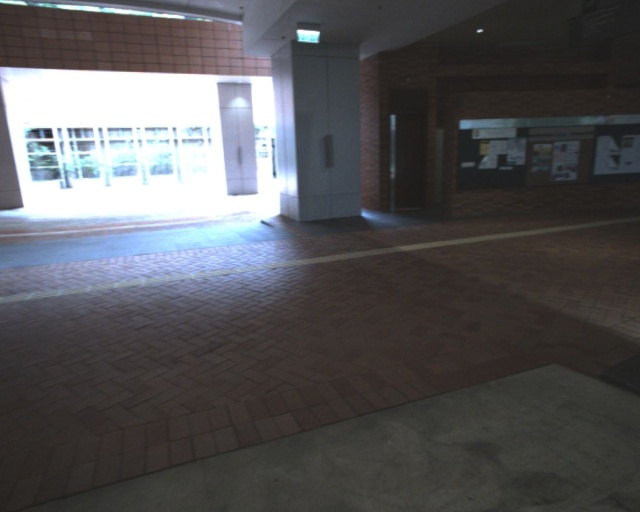
\includegraphics[width=0.188\textwidth]{../../images/compare-hku_campus_00/gt/test_0690.jpg} &
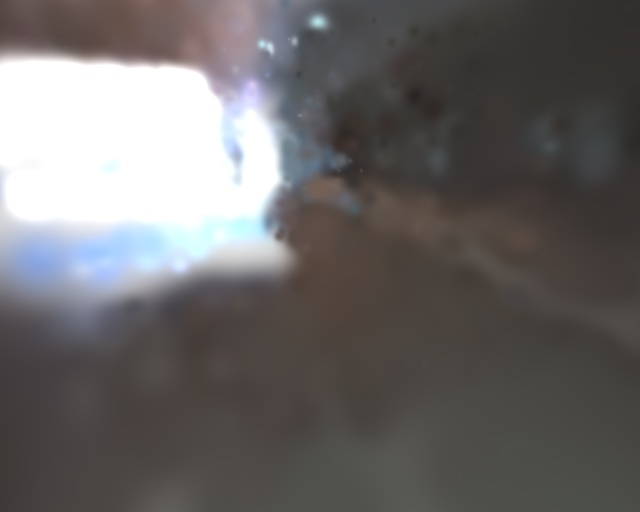
\includegraphics[width=0.188\textwidth]{../../images/compare-hku_campus_00/monogs/0690-test.jpg} &
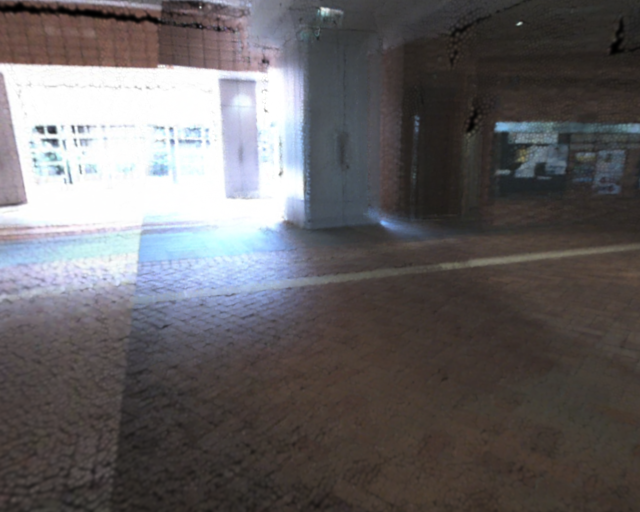
\includegraphics[width=0.188\textwidth]{../../images/compare-hku_campus_00/mm3dgs/test_0690.png} &
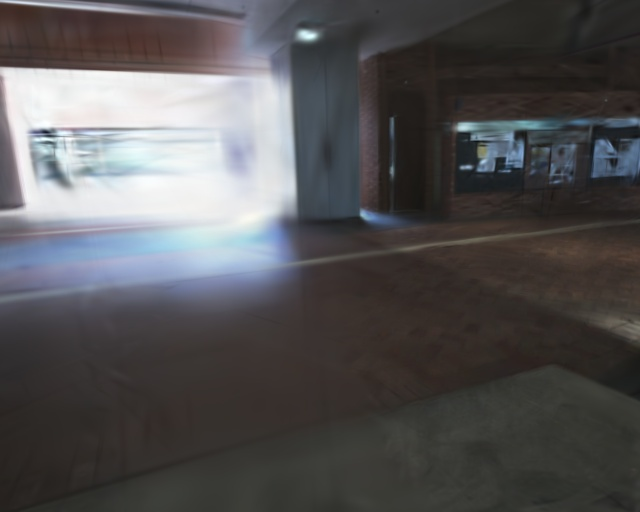
\includegraphics[width=0.188\textwidth]{../../images/compare-hku_campus_00/gslic2/test_0690.jpg} &
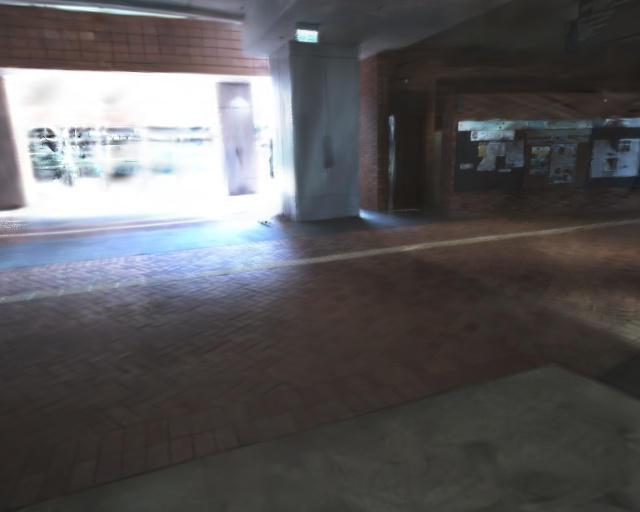
\includegraphics[width=0.188\textwidth]{../../images/compare-hku_campus_00/ours/test_0690.jpg} \\
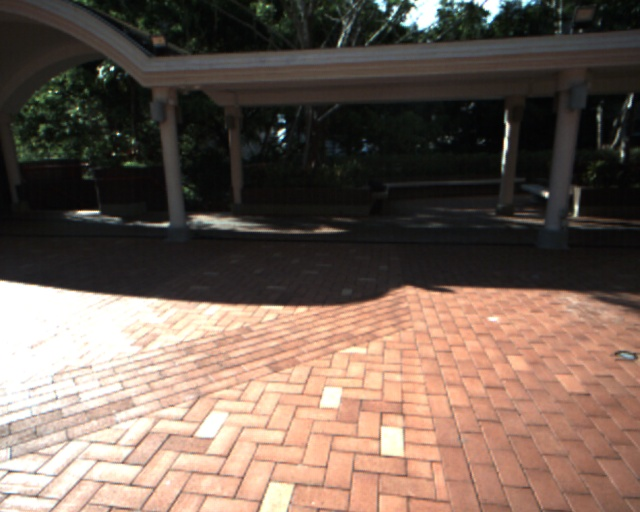
\includegraphics[width=0.188\textwidth]{../../images/compare-degenerate_00/gt/test_0516.jpg} &
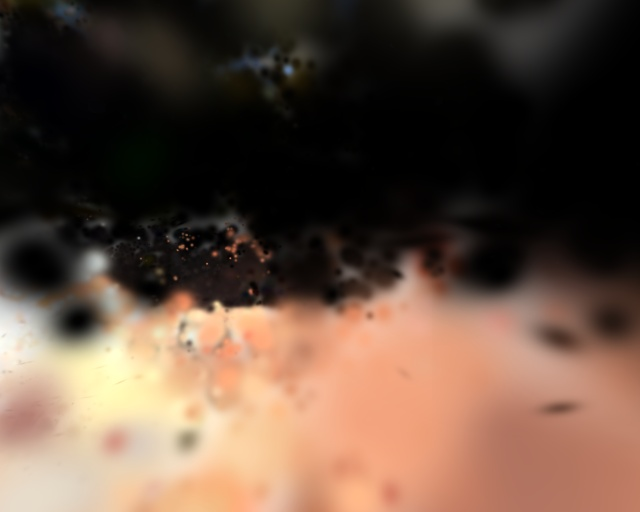
\includegraphics[width=0.188\textwidth]{../../images/compare-degenerate_00/monogs/0516-test.jpg} &
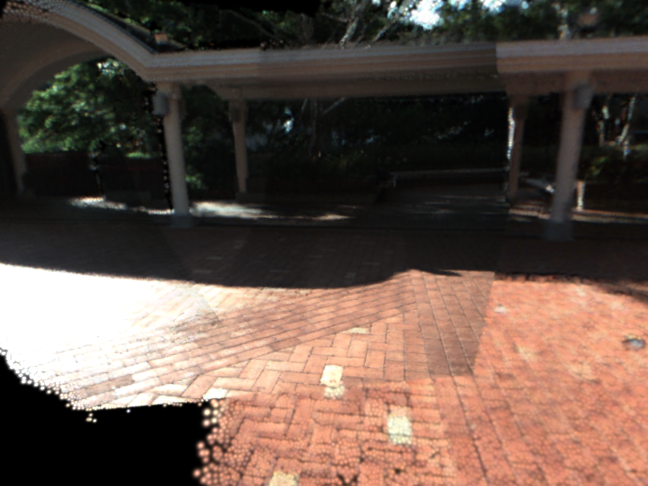
\includegraphics[width=0.188\textwidth]{../../images/compare-degenerate_00/mm3dgs/test_0516.png} &
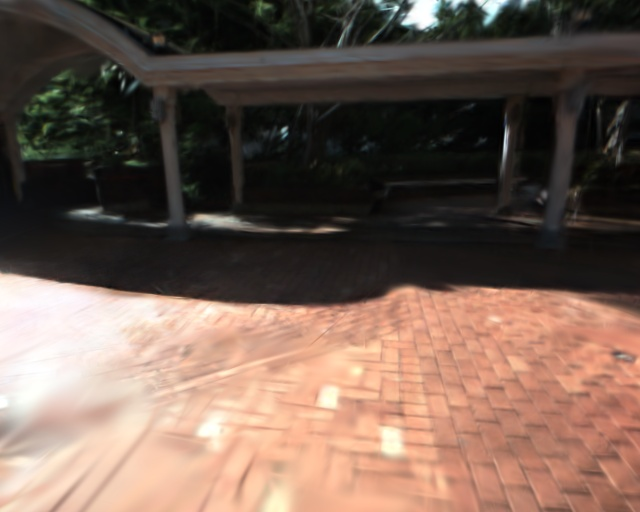
\includegraphics[width=0.188\textwidth]{../../images/compare-degenerate_00/gslic2/test_0516.jpg} &
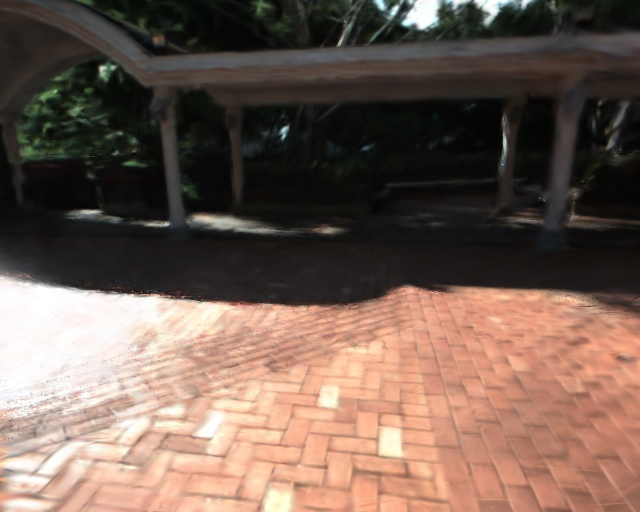
\includegraphics[width=0.188\textwidth]{../../images/compare-degenerate_00/ours/test_0516.jpg} \\
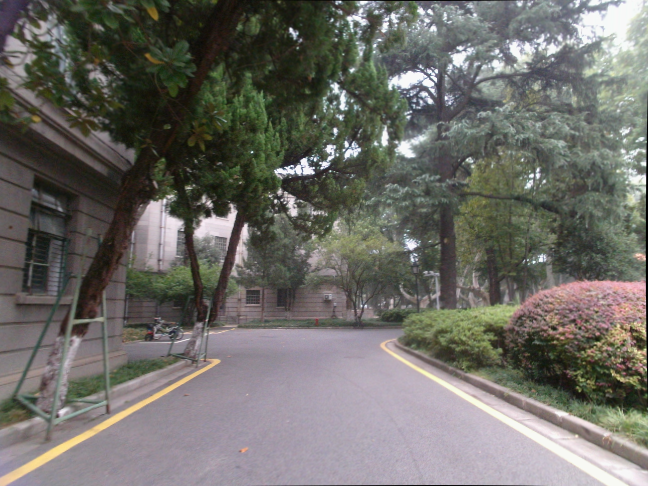
\includegraphics[width=0.188\textwidth]{../../images/compare-custom-2/gt/test_1080.png} &
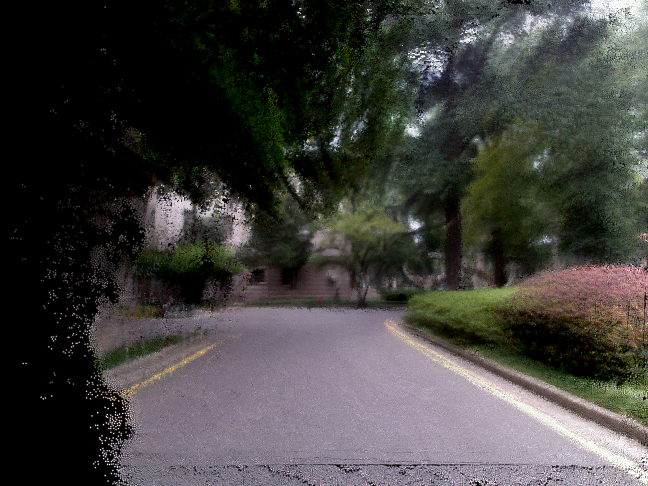
\includegraphics[width=0.188\textwidth]{../../images/compare-custom-2/monogs/test_1080.jpg} &
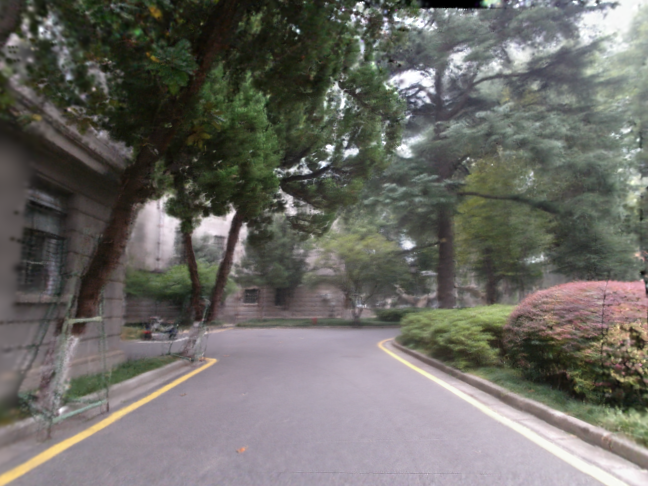
\includegraphics[width=0.188\textwidth]{../../images/compare-custom-2/mm3dgs/test_1080.png} &
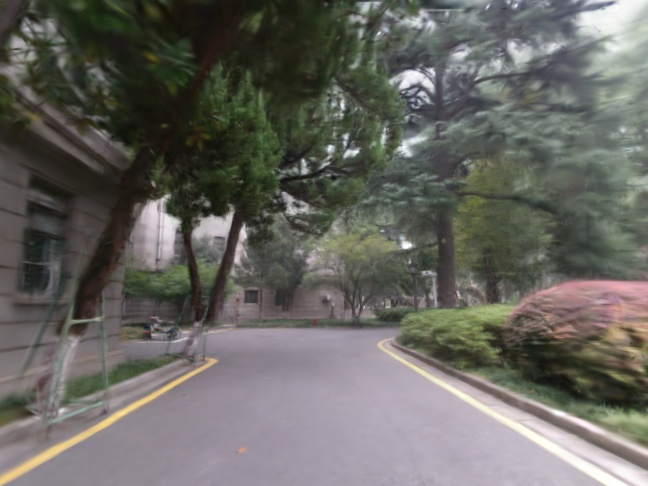
\includegraphics[width=0.188\textwidth]{../../images/compare-custom-2/gslic2/test_1080.jpg} &
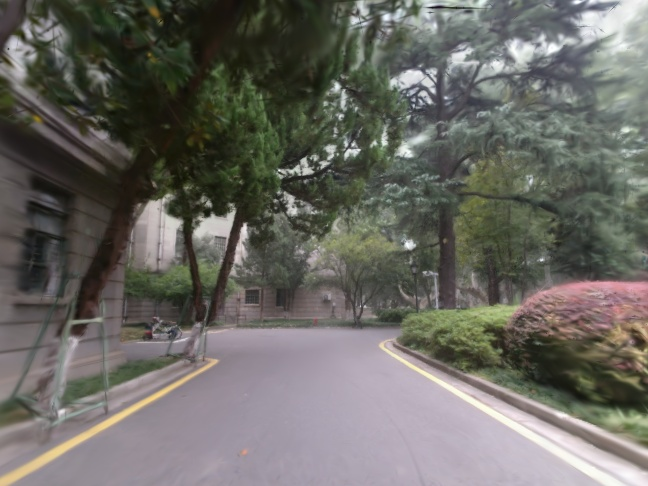
\includegraphics[width=0.188\textwidth]{../../images/compare-custom-2/ours/test_1080.jpg} \\
\end{tabular}
\caption{Qualitative comparison on public and self-collected datasets. Row 1: \texttt{hku\_campus\_00} frame 690. Row 2: \texttt{degenerate\_seq\_00} frame 516. Row 3: \texttt{seu\_campus\_seq\_01} frame 1080. Compared with MonoGS, MM3DGS-SLAM, and Gaussian-LIC2, our method preserves sharper details at structural boundaries, ground textures, and distant regions, while significantly reducing blur, trailing artifacts, and local distortion.}
\label{fig:qualitative_compare}
\end{figure*}

\subsection{Ablation Study: Effect of the Feed-Forward Regressor}

To verify the contribution of the feed-forward regressor to incremental 2DGS mapping, we conduct an ablation study on \texttt{hku\_campus\_00}. We denote the system without the regressor (using rule-based initialization) as Baseline and the full system as Ours. Unlike comparisons on a few representative frames, we collect the optimization trajectories of all training frames and plot them against the number of post-insertion optimization steps (\texttt{train\_times}), evaluating from three angles: (i) early quality at a fixed optimization budget, (ii) overall convergence benefit within the first 16 steps (AUC), and (iii) the number of steps required to reach a given quality threshold. The PSNR, SSIM, and LPIPS thresholds are set to 25.0, 0.70, and 0.18, respectively.

\begin{table}[!t]
\centering
\caption{Ablation results on \texttt{hku\_campus\_00}. Statistics are computed over the optimization trajectories of all training frames. The first two rows report mean $\pm$ std at 16 steps; the middle two rows report the AUC over the first 16 steps; the last two rows report the mean $\pm$ std steps to reach the quality threshold, with the number of frames that successfully reach the threshold in parentheses.}
\label{tab:ablation_regressor}
\renewcommand{\arraystretch}{1.18}
\resizebox{\columnwidth}{!}{%
\begin{tabular}{lccc}
\toprule
\textbf{Setting} & \textbf{PSNR$\uparrow$} & \textbf{SSIM$\uparrow$} & \textbf{LPIPS$\downarrow$} \\
\midrule
Baseline (16 steps) & 23.97 $\pm$ 2.91 & 0.800 $\pm$ 0.071 & 0.213 $\pm$ 0.055 \\
Ours (16 steps) & \textbf{24.34 $\pm$ 2.74} & \textbf{0.813 $\pm$ 0.063} & \textbf{0.195 $\pm$ 0.048} \\
\midrule
Baseline (AUC@16) & 362.96 $\pm$ 44.54 & 12.251 $\pm$ 1.302 & 4.266 $\pm$ 0.978 \\
Ours (AUC@16) & \textbf{370.57 $\pm$ 40.43} & \textbf{12.475 $\pm$ 1.149} & \textbf{4.033 $\pm$ 0.866} \\
\midrule
Baseline (time-to-quality) & 20.4 $\pm$ 28.1 (255/391) & 3.2 $\pm$ 6.2 (373/391) & 27.0 $\pm$ 24.5 (257/391) \\
Ours (time-to-quality) & \textbf{17.7 $\pm$ 26.0 (281/391)} & \textbf{3.1 $\pm$ 10.2 (382/391)} & \textbf{19.6 $\pm$ 15.6 (323/391)} \\
\bottomrule
\end{tabular}%
}
\end{table}

Table~\ref{tab:ablation_regressor} shows that introducing the feed-forward regressor consistently improves early convergence across training frames. Under a fixed budget of 16 post-insertion optimization steps, Ours outperforms Baseline on all three rendering metrics and AUC statistics. Ours also reaches the target quality in fewer average steps, with a higher number of successfully converged frames under all three thresholds. Table~\ref{tab:ablation_curves} further lists the mean convergence trends of the three metrics over the first 16 optimization steps.

\begin{table}[!t]
\centering
\caption{Early convergence of the feed-forward regressor ablation on \texttt{hku\_campus\_00}. Values are averaged over valid training frames; bold indicates the better result at each step.}
\label{tab:ablation_curves}
\renewcommand{\arraystretch}{1.14}
\setlength{\tabcolsep}{4pt}
\resizebox{\columnwidth}{!}{%
\begin{tabular}{llccccc}
\toprule
\multirow{2}{*}{\textbf{Metric}} & \multirow{2}{*}{\textbf{Method}} & \multicolumn{5}{c}{\textbf{Steps after insertion}} \\
\cmidrule(lr){3-7}
 & & \textbf{0} & \textbf{4} & \textbf{8} & \textbf{12} & \textbf{16} \\
\midrule
PSNR$\uparrow$ & Baseline & 18.18 & 22.07 & 23.41 & 23.95 & 23.97 \\
 & Ours & \textbf{18.92} & \textbf{22.83} & \textbf{23.83} & \textbf{24.20} & \textbf{24.34} \\
\addlinespace[2pt]
SSIM$\uparrow$ & Baseline & 0.636 & 0.753 & 0.786 & 0.800 & 0.800 \\
 & Ours & \textbf{0.661} & \textbf{0.772} & \textbf{0.797} & \textbf{0.810} & \textbf{0.813} \\
\addlinespace[2pt]
LPIPS$\downarrow$ & Baseline & 0.380 & 0.291 & 0.248 & 0.226 & 0.213 \\
 & Ours & \textbf{0.366} & \textbf{0.276} & \textbf{0.233} & \textbf{0.211} & \textbf{0.195} \\
\bottomrule
\end{tabular}%
}
\end{table}

The visualization results in Fig.~\ref{fig:ablation_visual} provide an intuitive explanation for the improved early convergence. Without the regressor, initial Gaussian parameters are given by hand-crafted rules and exhibit strong randomness and disorder, requiring multiple optimization rounds to align with the scene. With the regressor, the scene layout and dominant structures are already recognizable at step 0. The regressor exhibits adaptive behavior across different regions: in under-reconstructed or poorly covered areas, the predicted Gaussians tend toward larger coverage to quickly fill in the dominant structure; in regions with adequate geometric support or rich detail, the predictions favor finer-grained Gaussians to avoid over-covering details. Similarly, in low-texture or large smooth areas, the regressor tends to produce larger Gaussians for efficient early coverage, whereas in regions with richer texture and denser structural boundaries, the predicted Gaussians are typically smaller and more concentrated to facilitate detail expression. As optimization proceeds, our method converges to clear and stable renderings more rapidly.

\newcommand{\ablimg}[1]{\includegraphics[width=0.144\textwidth]{#1}}

\begin{figure*}[!t]
\begin{center}
{\scriptsize
\setlength{\tabcolsep}{1pt}
\renewcommand{\arraystretch}{0.82}
\begin{tabular}{@{}c@{\hspace{2pt}}ccc@{\hspace{5pt}}ccc@{}}
& \multicolumn{3}{c}{Baseline} & \multicolumn{3}{c}{Ours} \\
frame & 0 steps & 4 steps & 8 steps & 0 steps & 4 steps & 8 steps \\
\texttt{0004} &
\ablimg{../../images/self_compare/baseline/train_0004/times_0000.jpg} &
\ablimg{../../images/self_compare/baseline/train_0004/times_0004.jpg} &
\ablimg{../../images/self_compare/baseline/train_0004/times_0008.jpg} &
\ablimg{../../images/self_compare/ours/train_0004/times_0000.jpg} &
\ablimg{../../images/self_compare/ours/train_0004/times_0004.jpg} &
\ablimg{../../images/self_compare/ours/train_0004/times_0008.jpg} \\
\texttt{0084} &
\ablimg{../../images/self_compare/baseline/train_0084/times_0000.jpg} &
\ablimg{../../images/self_compare/baseline/train_0084/times_0004.jpg} &
\ablimg{../../images/self_compare/baseline/train_0084/times_0008.jpg} &
\ablimg{../../images/self_compare/ours/train_0084/times_0000.jpg} &
\ablimg{../../images/self_compare/ours/train_0084/times_0004.jpg} &
\ablimg{../../images/self_compare/ours/train_0084/times_0008.jpg} \\
\texttt{0609} &
\ablimg{../../images/self_compare/baseline/train_0609/times_0000.jpg} &
\ablimg{../../images/self_compare/baseline/train_0609/times_0004.jpg} &
\ablimg{../../images/self_compare/baseline/train_0609/times_0008.jpg} &
\ablimg{../../images/self_compare/ours/train_0609/times_0000.jpg} &
\ablimg{../../images/self_compare/ours/train_0609/times_0004.jpg} &
\ablimg{../../images/self_compare/ours/train_0609/times_0008.jpg} \\
\texttt{0784} &
\ablimg{../../images/self_compare/baseline/train_0784/times_0000.jpg} &
\ablimg{../../images/self_compare/baseline/train_0784/times_0004.jpg} &
\ablimg{../../images/self_compare/baseline/train_0784/times_0008.jpg} &
\ablimg{../../images/self_compare/ours/train_0784/times_0000.jpg} &
\ablimg{../../images/self_compare/ours/train_0784/times_0004.jpg} &
\ablimg{../../images/self_compare/ours/train_0784/times_0008.jpg} \\
\end{tabular}
}
\end{center}
\caption{Ablation visualization of the feed-forward regressor. Representative frames \texttt{train\_0004}, \texttt{train\_0084}, \texttt{train\_0609}, and \texttt{train\_0784} are shown after 0, 4, and 8 post-insertion optimization steps. Left three columns: Baseline; right three columns: Ours.}
\label{fig:ablation_visual}
\end{figure*}

The experiments lead to two conclusions. First, in the full novel-view rendering evaluation, our method outperforms all baselines on every test sequence, demonstrating that combining 2DGS representation with context-aware feed-forward insertion consistently improves the rendering quality of incremental Gaussian maps. Second, the core value of the feed-forward regressor lies not merely in slightly higher final metrics but in the significant improvement of the initial quality and early convergence speed after new Gaussian insertion. This property is particularly important for online systems, because better initial Gaussians not only reduce local artifacts but also provide more reliable rendering supervision for subsequent frames, creating a positive feedback loop that continuously improves the overall map quality.

%%%%%%%%%%%%%%%%%%%%%%%%%%%%%%%%%%%%%%%%%%%%%%%%%%%%%%%%%%%%%%%%%%%%%%%%%%%%%%%%
% V. CONCLUSION
%%%%%%%%%%%%%%%%%%%%%%%%%%%%%%%%%%%%%%%%%%%%%%%%%%%%%%%%%%%%%%%%%%%%%%%%%%%%%%%%

\section{CONCLUSION}

We address the problem that the initial quality of newly inserted Gaussians determines the cumulative mapping result in incremental scene reconstruction and propose a context-aware feed-forward Gaussian regression system based on 2DGS surfels. The method fuses contextual information with geometric priors to directly predict new surfel attributes at the insertion stage, replacing traditional rule-based initialization. The network is trained through self-distillation without additional annotated data.

Experiments on R3LIVE and MCD demonstrate that the proposed method consistently improves novel-view rendering quality of incremental Gaussian maps, achieving an average improvement of 1.28\,dB PSNR on R3LIVE over the closest multi-sensor baseline. Ablation studies further show that the main benefit comes from improved initial surfel state and early convergence quality, a property that is particularly valuable for online mapping under constrained optimization budgets. The current method still relies on a stable external front-end; future work will explore incremental Gaussian mapping under weaker prior conditions.

\addtolength{\textheight}{-6cm}

%%%%%%%%%%%%%%%%%%%%%%%%%%%%%%%%%%%%%%%%%%%%%%%%%%%%%%%%%%%%%%%%%%%%%%%%%%%%%%%%
% REFERENCES
%%%%%%%%%%%%%%%%%%%%%%%%%%%%%%%%%%%%%%%%%%%%%%%%%%%%%%%%%%%%%%%%%%%%%%%%%%%%%%%%

\bibliographystyle{ieeetr}
\bibliography{references}

\end{document}
